\section{Evaluation}
\label{sec: evaluation}

In this section, we present AdaCompress's behavior and effectiveness by some real-world experiments. %% \\

\subsection{Experiment Setup}

We carry out real-world experiments to verify our solution's performance. We use a desktop PC with an NVIDIA 1080ti graphic card as the edge infrastructure. For the cloud deep learning services, we choose Baidu Vision, Face++ object detection services, and Amazon Rekognition. In the experiments, we use two datasets mentioned before in Sec.~\ref{subsec:insight}, ImageNet dataset indicating daytime scenery and the FLIR Thermal Dataset indicating nighttime scenery. Some important hyperparameters in our experiments are given in Table ~\ref{tab: parameters}.

\begin{table}[H]
    \centering
    %     \begin{tabular}{llllll}
    \begin{tabular}{cccccc}
        \toprule
        notation          & value & & & notation     & value  \\ \midrule
        $c_{\rm ref}$ & 75    & & & $K$      & 1000   \\
        $\epsilon_{\min}$    & 0.02  & & & $p_0$    & 0.2    \\
        $\gamma$      & 0.95  & & & $\omega$ & -3   \\
        $ \mu_{\rm dec} $ & 0.99 & & & $ T $ & 5  \\
        $r_{\rm th}$  & 0.45   & & &   $ n  $  &  10      \\ \bottomrule
    \end{tabular}
    \caption{Experiment parameter settings}
    \label{tab: parameters}
    %     \vspace{-0.3cm}
\end{table}

\subsection{Dataset}

We use two datasets, the ImageNet dataset and the FLIR Thermal Dataset. The Imagenet dataset is a Large-Scale Hierarchical Image, in which each node of the hierarchy is depicted by hundreds and thousands of images. Its images are mostly taken in the daytime, and therefore we use it as a daytime scenery. Usually, a surveillance camera captures colored images in the daytime and gray-scaled thermal images in the nighttime. Therefore we choose a thermal image dataset to act as a nighttime image dataset. The FLIR Thermal Dataset is such a dataset having more than 14000 images collected by thermal sensors.

We use the ImageNet dataset in size reduction and accuracy performance experiment, DeepN-JPEG comparative experiment, and end-to-end latency simulation. Moreover, we use ImageNet and the FLIR Thermal Dataset alternately to simulate the scenery change in the \emph{inference-estimation-querying-retraining} mechanism experiment, and analyze the RL agent's best compression strategy selection in different input image ``sceneries''.

\subsection{Metrics}
\label{subsec:metrics}

The default compression quality level for JPEG is usually 75~\cite{pillow_benchmark,imgmin}, therefore we regard this as a typical value $ c_{\rm ref} = 75 $ of the conventional benchmark. %% \\

In our experiments, we measure the compressed and original image's file size to obtain the compression rate $ \Delta s $. Since we don't have the real ground truth label of an image, we use the output $ \vec{y}_{\rm ref} $ from a reference image as the ground truth label, and calculate the relative top-5 accuracy $ \mathcal{A} $ as the accuracy metric, the formula of $ \mathcal{A} $ is presented in Sec.~\ref{subsec: formulation}.

\subsection{Upload Image Size Overhead}

\begin{figure}[htbp]
    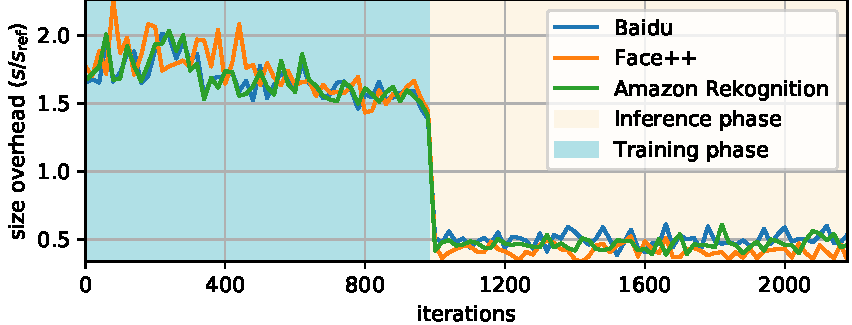
\includegraphics[width=\linewidth]{figures/train_steps_new.pdf}
    \caption{Size overhead in training and inference phase}
    \label{fig: train_steps}
    % \vspace{-0.3cm}
\end{figure}

Figure~\ref{fig: train_steps} presents the upload traffic load of the training and inference phase, to be more intuitionistic, we plot the size overhead $ \frac{s}{s_{\rm ref}} $ as the $ y $-axis where $ s $ is the real upload size of AdaCompress, $ s_{\rm ref} $ is the benchmark upload size. Therefore $ y \geq 1 $ means that our solution uploads more data then benchmark, and $ y < 1 $ means the compression rate of AdaCompress. From Figure~\ref{fig: train_steps} we can see that as the training procedure runs, the upload image size decreases because the RL agent learns to choose better compression quality levels to upload fewer data. In the training phase, to train the agent while remaining a convincing recognition result, we have to upload the original image to the cloud to get the real result, along with the compressed image to obtain reward feedback, therefore the upload traffic load is even higher than the conventional solution. But once the training phase has finished, the upload traffic load is lower than the benchmark. As shown in Figure~\ref{fig: compress_performance}, in the inference phase, AdaCompress's upload size is only 1/2 of the benchmark's. %% \\

\subsection{Size Reduction and Accuracy Performance}

\begin{figure}[htbp]
    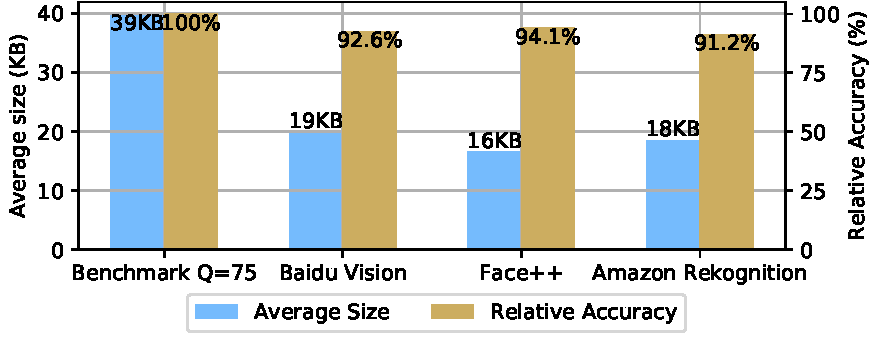
\includegraphics[width=\linewidth]{figures/compress-performance.pdf}
    \caption{Average size and relative accuracy on different cloud services}
    \label{fig: compress_performance}
    % \vspace{-0.3cm}
\end{figure}

Figure~\ref{fig: compress_performance} presents the compression performance in the inference phase for each cloud service. We test AdaCompress on Face++, Baidu Vision and Amazon Rekognition, comparing to the conventional compression level, for all tested cloud services, our solution can reduce the upload size by more than 1/2, meanwhile, the relative accuracy, indicated by brown bars, only decreases about 7\% on average, proving the efficiency of our design. %% \\

\subsection{DeepN-JPEG Comparative Experiment}

\begin{figure}[htbp]
    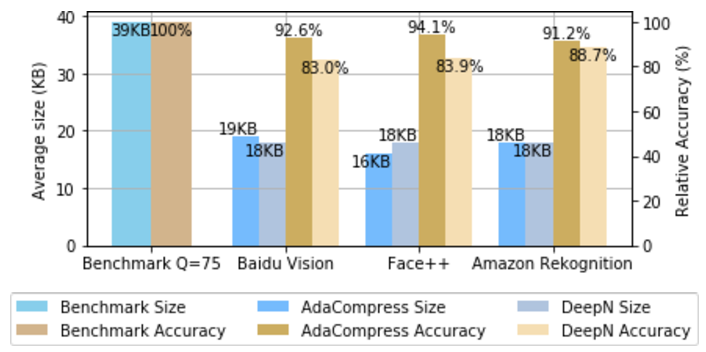
\includegraphics[width=\linewidth]{figures/compare_DeepN.pdf}
    \caption{Comparative compression performance between DeepN-JPEG and AdaCompress}
    \label{fig: compare_DeepN}
    % \vspace{-0.3cm}
\end{figure}

\begin{figure*}[htbp]
    \begin{minipage}{0.3\linewidth}
        \centerline{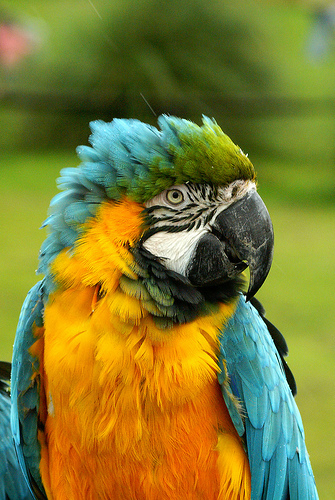
\includegraphics[width=4.0cm,trim=0 80 0 100,clip ]{figures/parrot_q75.jpeg}}
        \centerline{(1a) Origin Image (Q=75)}
        \centerline{Baidu prediction \ = \ ["parrot"]}
    \end{minipage}
    \hfill
    \begin{minipage}{0.2\linewidth}
        \centerline{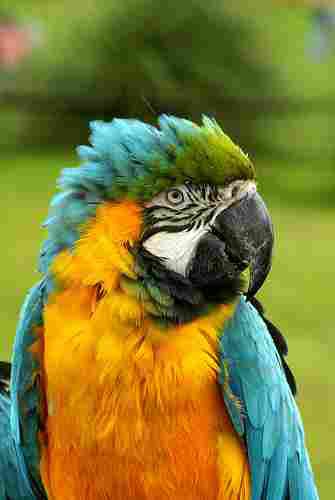
\includegraphics[width=4.0cm,trim=0 80 0 100,clip ]{figures/parrot_q15.jpeg}}
        \centerline{(1b) AdaCompress (choose Q=15)}
        \centerline{Baidu prediction \ = \ ["parrot"]}
    \end{minipage}
    \hfill
    \begin{minipage}{0.3\linewidth}
        \centerline{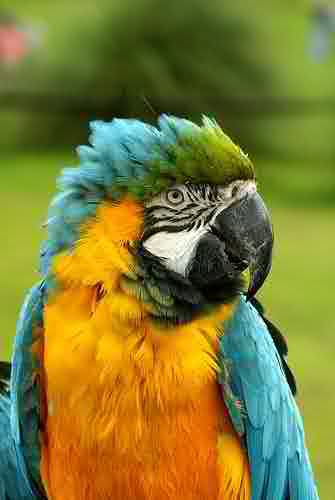
\includegraphics[width=4.0cm,trim=0 80 0 100,clip ]{figures/parrot_deepn.jpeg}}
        \centerline{(1c) DeepN-JPEG}
        \centerline{Baidu prediction \ = \ ["parrot"]}
    \end{minipage}
    
    \vfill
    \vspace{0.4cm}
    
    \begin{minipage}{0.3\linewidth}
        \centerline{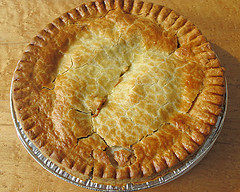
\includegraphics[width=4.0cm,trim=0 0 0 0,clip ]{figures/cake_q75.jpeg}}
        \centerline{(2a) Origin Image (Q=75)}
        \centerline{Baidu prediction \ = \ ["cake"]}
    \end{minipage}
    \hfill
    \begin{minipage}{0.2\linewidth}
        \centerline{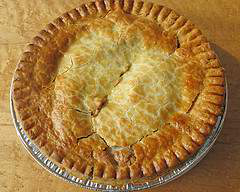
\includegraphics[width=4.0cm,trim=0 0 0 0,clip ]{figures/cake_q65.jpeg}}
        \centerline{(2b) AdaCompress (choose Q=65)}
        \centerline{Baidu prediction \ = \ ["cake"]}
    \end{minipage}
    \hfill
    \begin{minipage}{0.3\linewidth}
        \centerline{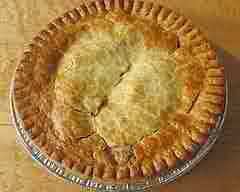
\includegraphics[width=4.0cm,trim=0 0 0 0,clip ]{figures/cake_deepn.jpeg}}
        \centerline{(2c) DeepN-JPEG}
        \centerline{Baidu prediction \ = \ ["fossil"]}
    \end{minipage}
    \vspace{0.2cm}
    \caption{Comparative compressed images of DeepN-JPEG and AdaCompress}
    \label{fig: compare_image}
\end{figure*}

Figure~\ref{fig: compare_DeepN} presents a comparison performance between DeepN-JPEG and AdaCompress for each cloud service. As we can see, both DeepN-JPEG and AdaCompress cut down the upload size overhead more than 1/2. However, for all tested cloud services, AdaCompress's accuracy is higher than DeepN-JPEG's slightly. Compared with DeepN-JPEG's average accuracy is about 85\% on three cloud services, while AdaCompress achieves a better average accuracy of 93\%. In a word, comparing to the DeepN-JPEG framework, AdaCompress presents a similar upload traffic load reduction performance but achieving higher inference accuracy for online computer vision-based services.

AdaCompress compresses images in a more adaptive manner rather than DeepN-JPEG. (i.e., the explanation of why AdaCompress achieves a better accuracy). As shown in Figure~\ref{fig: compare_image}, for picture 1a, compared to DeepN-JPEG, AdaCompress compresses the image at the compression quality level of 15, a more aggressive compression quality level to reduce upload size overhead. On the contrary, for picture 2a of Figure~\ref{fig: compare_image}, DeepN-JPEG compresses the image with the same quantization table, but AdaComperss chooses a higher compression quality level to preserve more details so that the backend deep learning model can still recognize the picture. Being different from the DeepN-JPEG framework compresses all images with the same quantization table, our RL agent chooses a lower compression quality level for picture 1a and a relatively higher compression quality level for picture 2a based on the feature of the input image. 

%Comparing to DeepN-JPEG, AdaCompress compresses images more adaptively for different images and cloud computer vision services to achieve higher accuracy, while maintaining a similar average upload size overhead.

Comparing to DeepN-JPEG, AdaCompress has three advantages and one disadvantage as following: %% \\    
    \begin{itemize}
        \item AdaCompress and DeepN-JPEG both decrease the upload size overhead more than 1/2, but AdaCompress maintains higher inference accuracy.
        \item DeepN-JPEG requires the original dataset information to re-design the quantization table, while AdaCompress chooses compression quality level adaptively without any pre-knowledge of the original dataset. 
        \item When the scenery changes, DeepN-JPEG still compresses images with the same quantization table, while AdaCompress's \emph{inference-estimation-querying-retraining} mechanism captures the scenery change and invokes either model querying method or retraining kernel to \emph{generate} a more suitable compression selection strategy for the current scenery.
        \item DeepN-JPEG re-designs the quantization table \emph{locally}, while AdaCompress needs to upload origin images and compressed images to the cloud in the training phase, leading some upload size overhead at the beginning. 
    \end{itemize}

\subsection{Adaptively Cope With the Scenery Change}

To evaluate the efficiency of the \emph{inference-estimation-querying-retraining} mechanism, we feed AdaCompress with a combined dataset whose first 2000 images from FLIR Thermal images, the later 3000 images randomly sampled from ImageNet, and the last 2000 images from FLIR Thermal images. We adapt AdaCompress's current RL agent to FLIR Thermal nighttime scenery by training it on the FLIR dataset, and we run AdaCompress on the combined dataset, observing AdaCompress's behavior upon the scenery changes at step 2000 and 5000. %% \\

We illustrate AdaCompress's behavior in Figure~\ref{fig: running-retrain}, the $ x $-axis indicates steps, the vertical red line means the dataset change (i.e. scenery change). We plot AdaCompress's overall accuracy as the green line and the estimation probability $ p_{\rm est} $ as the gray line. At the bottom of Figure~\ref{fig: running-retrain}, we also plot the scaled upload size of AdaCompress and benchmark solution to illustrate the upload size overhead in the inference phase.
%with a $ \Delta $ mark on $ x $-axis

%\begin{figure}[htbp]
%    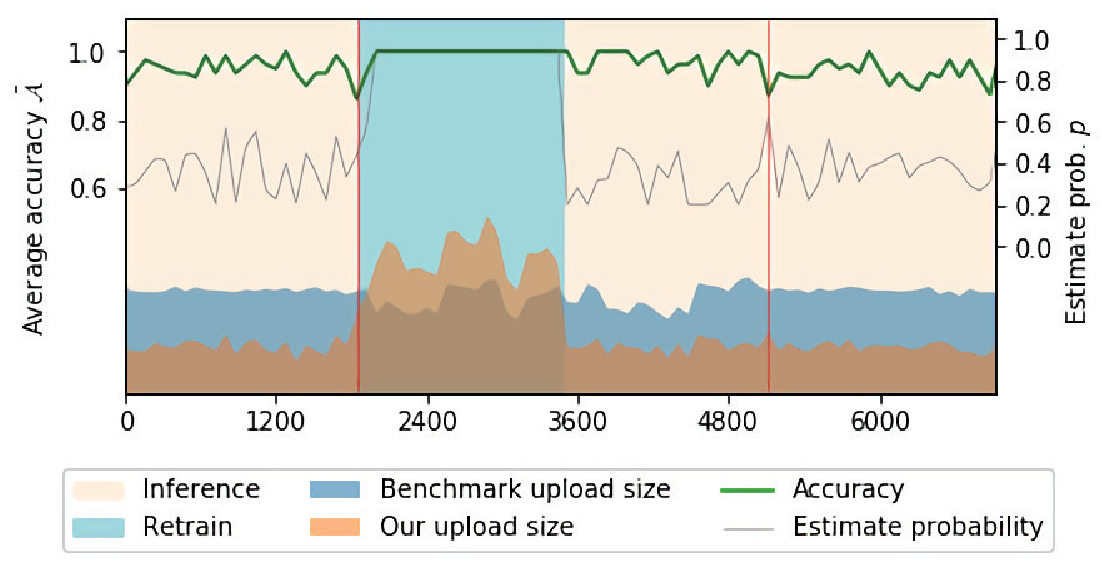
\includegraphics[width=\linewidth]{figures/running-retrain.pdf}
%    \caption{AdaCompress's reaction upon scenery change}
%%    \vspace{-0.2cm}
%    \label{fig: running-retrain}
%\end{figure}
\begin{figure}[H]
    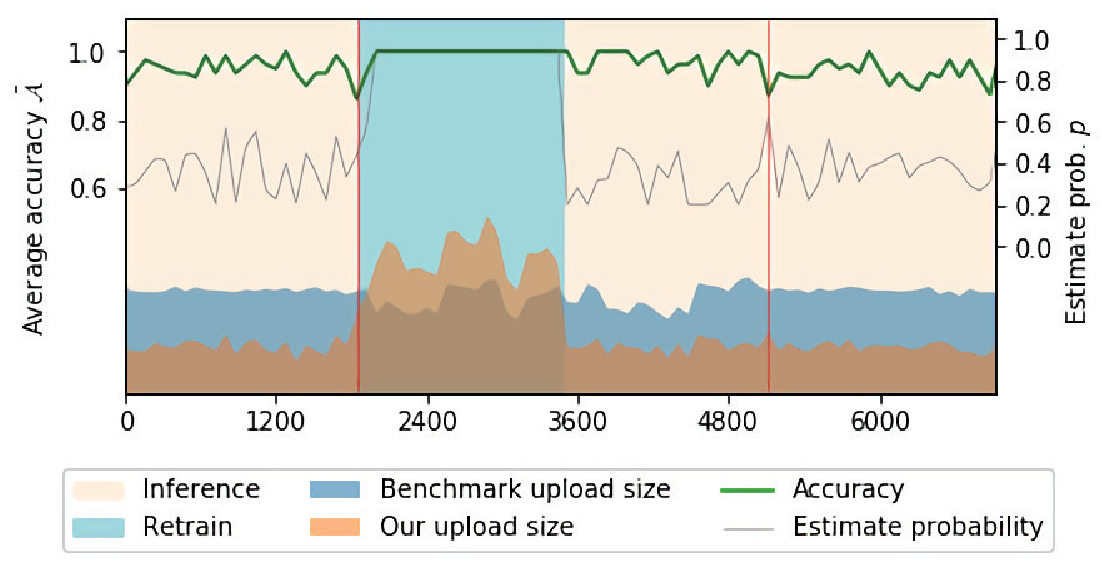
\includegraphics[width=\linewidth]{figures/running-retrain.pdf}
    \caption{AdaCompress's reaction upon scenery change}
    %    \vspace{-0.2cm}
    \label{fig: running-retrain}
\end{figure}

From Figure~\ref{fig: running-retrain} we can see that AdaCompress can adaptively update the estimation probability $ p_{\rm est} $, usually, when the overall accuracy decreases, AdaCompress would increase the estimation probability, trying to capture the scenery change. When the overall accuracy is stable and high enough, the estimation probability $ p_{\rm est} $ decreases to reduce transmission. %% \\

Upon the first data scenery changes (i.e., night to day) shown as the first vertical red line in Figure~\ref{fig: running-retrain}, comparing to the earlier steps, the accuracy decreases dramatically and therefore $ p_{\rm est} $ raises to determine whether the scenery changes. The accuracy keeps dropping in the following estimations, indicating that the current RL agent is no more suitable for the current input scenery. At the moment, AdaCompress should switch into the model querying state and re-load a new RL agent model from the model caching library. However, there is no model except the current RL agent in the model caching library at that time. Therefore, AdaCompress starts to re-train at once, to adapt the RL agent into the current scenery. The re-training steps are shown as the light-blue region in Figure~\ref{fig: running-retrain}. In the re-training phase, AdaCompress uses the reference image's prediction label $ \vec{y}_{\rm ref} $ as the output result, therefore the accuracy $ \mathcal{A} $ and $ p_{\rm est} $ are locked to 1. After finishing re-training the agent in the daytime scenery, the trained agent is cached in the model cachling library, and in the following iterations, sometimes the accuracy decreases accidentally, and the estimation probability $ p_{\rm est} $ also raises to get more samples. The accuracy is not lower than the accuracy threshold $ \mathcal{A}_0 $ , therefore the re-training phase would not be triggered again until the second data scenery changes. %% \\

Upon the second data scenery changes (i.e., day to night) shown as the second vertical red line in Figure~\ref{fig: running-retrain}, like the first scenery change, the accuracy decreases and $ p_{\rm est} $ raises, indicating that the current RL agent is no more suitable again. AdaCompress switches into the model querying state at once and re-loades a new RL agent model (i.e., the initial model trained on the FLIR Thermal images) from the model caching library. When using the new agent in this scenery, the accuracy stops decreasing and maintains above the accuracy threshold, indicating the current RL agent is suitable for the current scenery.  %% \\

From Figure~\ref{fig: running-retrain} we can also observe the uploading file size overhead in different phases, in re-training phase, AdaCompress uploads more data than the conventional benchmark, but in inference phase, AdaCompress's upload size is only half of the benchmark's. Especially when the second data scenery changes, AdaCompress achieves a lower upload traffic load by loading a suitable RL agent model rather than re-training from scratch. %% \\

\subsection{End-to-End Latency Simulation}

Comparing to the conventional solution that uploads the image directly, in our solution, the image is passed to the RL agent first to estimate the compression level. Running this RL agent brings extra latency to the whole system. In this subsection, we evaluate this latency overhead. %% \\

We test the RL agent's inference time and compressed file size for batches of images, and simulate the latency of uploading such compressed images. We test the average inference latency on 1000 ImageNet images and simulate the network bandwidth as 27.64 Mbps according to the global average fixed broadband upload speed~\cite{speedtest} in Feb. 2019, to verify the end-to-end latency performance. The latency comparison is listed in Table~\ref{tab: latency-overhead}. %% \\

\begin{table}[htbp]
    % \begin{table}[H]
    \centering
    %     \begin{tabular}{lll}
    \begin{tabular}{ccc}
        \toprule
        & Benchmark & AdaCompress  \\ \midrule
        Average upload size          & 42.68 KB  &  18.46 KB            \\
        Inference latency    & 0 s       & 2.09 ms          \\
        Transmission latency & 12.35 ms       & 5.34 ms          \\
        Overall latency      & 12.35 ms       & 7.43 ms          \\ \bottomrule
    \end{tabular}
    \caption{Latency between image upload and inference result feedback}
    \label{tab: latency-overhead}
    % \vspace{-0.5cm}
\end{table}

Our solution brings in inference latency to the end-to-end latency, but the transmission latency is much lower by shrinking the upload file size. In today's network architecture where the edge infrastructure's computational power is increasing significantly ~\cite{satyanarayanan2017emergence,hu2015mobile}, we can use the computing power of the edge infrastructure in exchange for the reduction of upload traffic load and transmission latency. %% \\
